\documentclass{article} % For LaTeX2e
\usepackage{cos424,times}
\usepackage{hyperref}
\usepackage{url}
\usepackage{float}

\usepackage{graphicx}


\usepackage{amsmath}
\usepackage{amssymb}
\usepackage{enumerate}
%\usepackage{fullpage}
%\usepackage[margin=0.5in]{geometry}
\usepackage{bbm}

\def \mcX {\mathcal{X}}
\def \mcY {\mathcal{Y}}
\def \mcH {\mathcal{H}}
\def \mcD {\mathcal{D}}

\def \P {\mathbb{P}}

\def \N {\mathbb{N}}
\def \Nbr {\mathcal{N}}
\def \Q {\mathbb{Q}}
\def \F {\mathbb{F}}
\def \then {\implies &}
\def \oif {\Longleftrightarrow &\,}
\def \given {\text{Given }&}
\def \assume {\text{Assume }&}
\def \thfr {\therefore &\enskip}
\def \bij {\leftrightarrow}
\def \inj {\rightarrowtail}
\def \sur {\twoheadedrightarrow}
\def \Z {\mathbb{Z}}
\def \R {\mathbb{R}}
\def \C {\mathbb{C}}
\def \iff {\Longleftrightarrow}
\def \kron {\boldsymbol\delta}
\def \indicator {\mathbbm{1}}

\def\Tx{\textbf{x}}
\def\Ty{\textbf{y}}
\def\quotient{\mathclose{}/\mathopen{}}
\def\Tf{\textbf{f}}
\def\Th{\textbf{h}}
\def\Tg{\textbf{g}}
\def\sumn{\sum_{n=0}^\infty}
\def\limn{\lim_{n\rightarrow\infty}}
\def\prodn{\prod_{n=0}^\infty}
\DeclareMathOperator\adj{adj}

\newcommand{\stc}[1]{\widetilde{#1}}   
\newcommand{\pa}[1]{ \left({#1}\right) }
\newcommand{\set}[2]{ \left\{ #1 \,\middle|\, #2 \right\} }
\newcommand{\shift}[1]{&\quad & \text{#1}\\}
\newcommand{\lem}[1]{\text{\textbf{L.\ref{#1}}}}
\newcommand{\card}[1]{\left\vert{#1}\right\vert}
\newcommand{\Ps}[1]{\mathcal{P}\left({ #1 }\right)}
\newcommand{\colv}[1]{\begin{pmatrix} #1 \end{pmatrix}}
\newcommand{\mat}[1]{\begin{pmatrix} #1 \end{pmatrix}}
\newcommand{\detmat}[1]{\begin{vmatrix} #1 \end{vmatrix}}
\newcommand{\spanb}[1]{\text{span}\{ #1 \}}
\newcommand{\abs}[1]{\left|#1\right|}
\newcommand{\Inner}[1]{\langle #1 \rangle}
\newcommand{\Innercpy}[1]{\langle #1, #1 \rangle}

\DeclareMathOperator{\Err}{\text{err}}
\DeclareMathOperator*{\ErrE}{\mathbb{E}}
\DeclareMathOperator{\Tr}{tr}
\DeclareMathOperator{\Dim}{dim}
\DeclareMathOperator{\Rank}{rank}
\DeclareMathOperator{\Ker}{ker}
\DeclareMathOperator{\Diam}{diam}
\DeclareMathOperator{\Int}{int}
\DeclareMathOperator{\Clo}{clo}
\DeclareMathOperator{\sgn}{sgn}
\DeclareMathOperator{\MyRe}{Re}
\DeclareMathOperator{\MyIm}{Im}


\title{COS 424 Homework 2}

\author{
Vladimir Feinberg\\
Princeton University\\
\texttt{vyf@princeton.edu}
}

\newcommand{\fix}{\marginpar{FIX}}
\newcommand{\new}{\marginpar{NEW}}

\begin{document}

\maketitle

\begin{abstract}
abstract
\end{abstract}

\section{Introduction and Related Work}

Imputation is a general statistical process involving replacing unknown values with a best guess based on a given context. Formally, we consider some vectors $\Tx_i\in S^n$ for some set $S$. If we take these $\Tx_i$ to be sampled from a distribution over $S^n$, we can make some predictions about the posterior of a $\Tx$ given some limited observation into a set of $\{\Tx_i\}$.

In our case, $S$ is a tuple over various biological information: chromosome number, genomic offset, strand type (3'-5' or 5'-3'), and methylation, the proportion of sites in a laboratory sample that had an additional methyl group attached to a cytosine molecule. The methylation count in our data set may be missing information.

Predicting whether the proportion of methylated sites from a sample is at least half has been done with over 90\% accuracy by relying on methylation levels of nearby sites, sequence-encoded information such as genetic context, and genomic position to the extent that the site is co-located (in the binary sense) with a DNA sequence for a particular protein or a sequence for a cis-regulartory element (CRE) \cite{zhang2015predicting}. Other studies have also found co-localization between CREs and CpGs (sites where the methylation occurs) \cite{ziller2013charting}.

\section{Exploratory Data Analysis}

We focus our analysis mainly on chromosome 1, which has samples from 379551 sites. There are 34 samples for each site, each taken from an expensive WGBS procedure, this method is able to measure about 91\% of sites \cite{laird2010principles}. Our test sample only has about 2\% of the sites available from a cheaper procedure: methylation microarrays \cite{zhang2015predicting}.

We are to use the limited information to impute the missing values in the sample. Because we can only use WGBS as the true value, there are some sites that we don't know the correct value for, even in testing. The imputation procedure may {\em not} be specified to only impute the sites we are testing for because this is a facet of our testing procedure. The methods constructed attempt to impute the entire genome. We are only able to provide an estimate for our testing error because we can only observe some of the true methylation values with the more expensive technique.

The sites available at test time are consistent - the technology used to assay the methylation values samples sites consistently \cite{infinium}. This opens up opportunities to take advantage of learning patterns particular to the sites consistently tested by the methylation microarrays - for instance, we can mask one of the well-sampled tissues enabling a sort of ``cross-validation" on a reduced feature set.

\begin{figure}[H]
    \centering
    
    \begin{minipage}[b]{0.3\textwidth}
        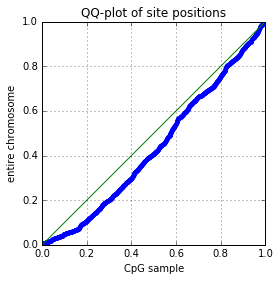
\includegraphics[width=\textwidth]{qqtest.png}
        %\caption{}
    \end{minipage}
    \hspace{0.15\textwidth}
    \begin{minipage}[b]{0.4\textwidth}
        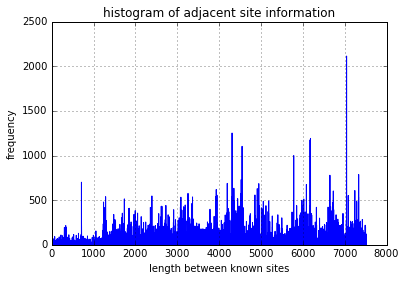
\includegraphics[width=\textwidth]{adjhist.png}
        %\caption{}
    \end{minipage}
    
    \label{fig:sampleknowndistrib}
    \caption{The above demonstrates the distribution of the known sites in the test sample. The mean distance between sites is 50.3, with a standard deviation of 87.0. The QQ-plot demonstrates that the sampling is fairly uniform throughout the chromosome.}
\end{figure}

The microarray may only provide about 2\% of the chromosome's information, but it may give enough to find chromosome-wide patterns as in Figure \ref{fig:sampleknowndistrib}. The uniformity here, coupled with the observations of correlation amongst neighboring sites from Figure \ref{fig:colocalsite} informs us local values may be informative.

\begin{figure}[H]
    \centering
    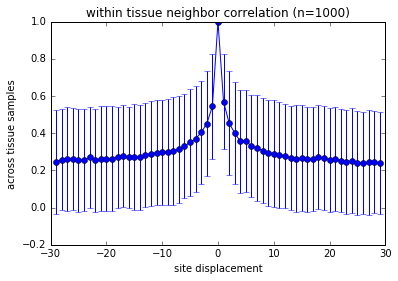
\includegraphics[width=0.4\textwidth]{colocalisitecorr.png}
    \label{fig:colocalsite}
    \caption{The above demonstrates estimates for the correlation of methylation values with the neighbours a given distance away from a sample site on the same tissue sample. The correlation across 33 of the 34 given tissues was taken. This was performed on 1000 random sites. The last chromosome was dropped due to its 98\% sparsity. The ``bottoming out" of correlation at about 0.25 as we distance ourselves from the site matches the observed background correlation from \cite{zhang2015predicting}. Error bars are $1\hat{\sigma}$.}
\end{figure}

We explore whether there's potential for (1) prediction based on genomic location or (2) prediction based on similarity to other chromosomes. Figure \ref{fig:genomictrends} shows the rolling mean of the methylation proportions - it confirms that while there are no obvious trends as a function of sequence, there are chromosomes with similar behavior.

\begin{figure}[H]
    \centering
    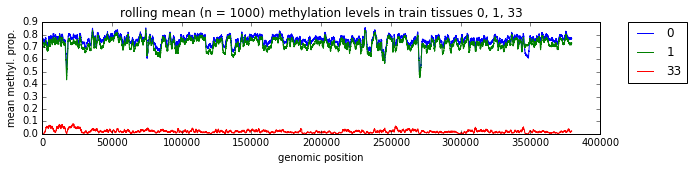
\includegraphics[width=0.9\textwidth]{genomictrends.png}
    \label{fig:genomictrends}
    \caption{Rolling mean with 1000 bp windows of methylation values for varying tissues. In order, the standard deviation ratio from the original tissue methylation values to the rolled mean ones are 4.83, 4.62, and 11.34. Note that this is the square root of the inverse of proportion of variance maintained by the rolling mean.}
\end{figure}

%TODO (once added) \CITE{} below too -> genetic context (intronic, ex, etc).
As recommended by \cite{zhang2015predicting}, additional info from the ENCODE project was retrieved, corresponding to the indicators that a given site is within the context of a transcription factor CRE. This introduces 161 binary features, which are used alongside the strand direction information as additional inputs compared to the other tissue methylation samples alone \cite{encode2004encode}.
\section{Methods}

Recall there are 34 sample tissues. Models were evaluated by average cross-validation performance by supplying 33 tissues with near-full methylation information and 1 sample with only the methylation sites revealed by the 2\%-sampling microarray mechanism \cite{infinium}. However, only 6 folds were performed, because certain tissue samples were sparse or highly uncorrelated with the any of the rest, and would be poor candidates for model selection for our test chromosome, see Figure \ref{fig:chromacorr}).

\begin{figure}[H]
    \centering
    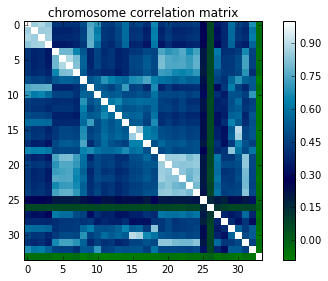
\includegraphics[scale=0.3]{chromacorr.png}
    \label{fig:chromacorr}
    \caption{Using only the training data, it was found that the closes training sample was chromosome 19. Thus, we estimate from the diagram above that chromosomes 19-24, inclusive, will be good folds to train our models on (by pretending they each only have limited methylation information).}
\end{figure} 

A fundamental assumption here is that the additional tissue data at test time on the holdout tissue sample will not significantly worsen the top model from cross-validation. This is a fair assumption since the model was selected with 33 similar features.

%TODO basic collab filtering (memory/similarity based, svd).
%TODO gmm with covar on local items
%TODO glm + look at coeffs to find predictive chromosomes. -> source for "similar methylation" if similar organs.
%TODO vector machine

\section{Results}

\section{Conclusion}


\subsubsection*{Acknowledgments}

The author would like to thank Prof. Engelhardt and Brian Jo for their advice on this project and Princeton University for access to certain references. %TODO thank encode.

\bibliographystyle{acm}
\bibliography{ref}

\end{document}
